%\documentclass[a4paper,12pt]{article}
%\usepackage[T1]{fontenc}
%\usepackage{imakeidx}
%\usepackage{graphicx}
%\makeindex[columns=3, title=Alphabetical Index, intoc]
%\usepackage{graphicx,wrapfig,lipsum}
%
%\usepackage[hmargin=3cm, vmargin=3cm]{geometry}
%\usepackage[font=tiny, labelfont=sc]{caption}
%
%\usepackage{listings}
%\usepackage{color}
%\usepackage{textcomp}
%\definecolor{listinggray}{gray}{0.9}
%\definecolor{lbcolor}{rgb}{0.9,0.9,0.9}
%\lstset{
%	backgroundcolor=\color{lbcolor},
%	tabsize=4,
%	rulecolor=,
%	language=matlab,
%        basicstyle=\scriptsize,
%        upquote=true,
%        aboveskip={1.5\baselineskip},
%        columns=fixed,
%        showstringspaces=false,
%        extendedchars=true,
%        breaklines=true,
%        prebreak = \raisebox{0ex}[0ex][0ex]{\ensuremath{\hookleftarrow}},
%        frame=single,
%        showtabs=false,
%        showspaces=false,
%        showstringspaces=false,
%        identifierstyle=\ttfamily,
%        keywordstyle=\color[rgb]{0,0,1},
%        commentstyle=\color[rgb]{0.133,0.545,0.133},
%        stringstyle=\color[rgb]{0.627,0.126,0.941},
%}
%
%
%
%\newcommand{\wrapfill}{\par\ifnum\value{WF@wrappedlines}>0
%  \addtocounter{WF@wrappedlines}{-1}%
%  \null\vspace{\arabic{WF@wrappedlines}\baselineskip}%
%  \WFclear
%\fi}
%
%
%\usepackage{ulem}
%

\documentclass[a4paper,12pt]{book}
\usepackage{color}
\usepackage[x11names]{xcolor}
\usepackage[usenames,dvipsnames,svgnames,table]{xcolor}
\usepackage{listings}
\usepackage[T1]{fontenc}
\usepackage{imakeidx}
\usepackage{graphicx}
%\makeindex[columns=3, title=Alphabetical Index, intoc]
\usepackage{graphicx,wrapfig,lipsum}

\usepackage[hmargin=1cm, vmargin=3cm]{geometry}
\usepackage[font=tiny, labelfont=sc]{caption}
\usepackage{hyperref}

%\usepackage{refcount}


%hyperlinks, coloured menu, submenu with different colors, clickable references
\hypersetup{
     colorlinks   = true,
     citecolor    = gray
}

\usepackage{tocloft}

\renewcommand{\cftsubsecfont}{\normalfont\hypersetup{linkcolor=cyan}}
\renewcommand{\cftsubsecafterpnum}{\hypersetup{linkcolor=green}}

\newcommand{\wrapfill}{\par\ifnum\value{WF@wrappedlines}>0
  \addtocounter{WF@wrappedlines}{-1}%
  \null\vspace{\arabic{WF@wrappedlines}\baselineskip}%
  \WFclear
\fi}


\author{
  Daniele, Della Cioppa\\
  \texttt{daniele.dellacioppa@gmail.com}
}
\title{Usage of the \texttt{\textbackslash author} command}

\renewcommand{\footnotesize}{\scriptsize}


%for chinese characters - not working yet
\usepackage{CJKutf8}
\usepackage[utf8]{inputenc} % optional
\usepackage[T1]{fontenc}


% for underlining
\usepackage{ulem}


%\usepackage{fontspec}

%\newfontfamily{\cfont}{Microsoft YaHei}


%nome del capitolo ad ogni pagina 
\usepackage{fancyhdr}
\pagestyle{fancy}

\fancyhf{}
\fancyhead[RO,LE]{\textbf{\thepage}}
\fancyhead[LO]{\nouppercase{\textbf{\color{teal}\leftmark}}}
\fancyhead[RE]{\nouppercase{\textbf{\color{cyan}\rightmark}}}

%possibility to add chapters

\usepackage[english]{babel}

%background image to parts
\usepackage{eso-pic}

\usepackage{sectsty}    %package to define colors
\definecolor{MarroncinoMH}{rgb}{0.4,0.4,0.25} %defining color
\definecolor{Bluettino}{rgb}{0.1,0.5,0.8} %defining color
\definecolor{Bluettetto}{rgb}{0.1,0.4,0.4} %defining color

\chapterfont{\color{MarroncinoMH}}   %using the defined color for chapter fonts
\sectionfont{\color{Bluettetto}}  %defining section color
\subsectionfont{\color{Bluettino}} %defining subsection color
\subsubsectionfont{\color{teal}} %defining subsection color
\paragraphfont{\color{OliveGreen}} %defining paragraph color
\subparagraphfont{\color{LimeGreen}} %defining subparagraph color


%coding blocks
\definecolor{listinggray}{gray}{0.9}
\definecolor{lbcolor}{rgb}{0.9,0.9,0.9}
\lstset{
	backgroundcolor=\color{lbcolor},
	tabsize=4,
	rulecolor=,
	language=matlab,
        basicstyle=\scriptsize,
        upquote=true,
        aboveskip={1.5\baselineskip},
        columns=fixed,
        showstringspaces=false,
        extendedchars=true,
        breaklines=true,
        prebreak = \raisebox{0ex}[0ex][0ex]{\ensuremath{\hookleftarrow}},
        frame=single,
        showtabs=false,
        showspaces=false,
        showstringspaces=false,
        identifierstyle=\ttfamily,
        keywordstyle=\color[rgb]{0,0,1},
        commentstyle=\color[rgb]{0.133,0.545,0.133},
        stringstyle=\color[rgb]{0.627,0.126,0.941},
}


%quoting
\usepackage{csquotes}

%epigraph
\usepackage{epigraph} 

%fonts
%\usepackage[T1]{fontenc}
%\usepackage{accanthis}


\usepackage{afterpage}

\makeatletter
% Macro \changepagecolor has the same syntax as \pagecolor or \color
% with an optional argument and a mandatory argument.
\newcommand*{\changepagecolor}{%
  \@ifnextchar[\@changepagecolor@i\@changepagecolor@ii
}
% Case: \changepagecolor[...]{...}
\def\@changepagecolor@i[#1]#2{%
  \@changepagecolor@do{[{#1}]{#2}}%
}
% Case: \changepagecolor{...}
\newcommand*{\@changepagecolor@ii}[1]{%
  \@changepagecolor@do{{#1}}%
}
\newcommand*{\@changepagecolor@do}[1]{%
  % Fill the remaining space with a colored rule
  \begingroup
    \offinterlineskip
    \hbox to 0pt{%
      \kern-\paperwidth
      \vtop to 0pt{%
        \color#1%
        \hrule width 2\paperwidth height \paperheight
        \vss
      }%
      \hss
    }%
  \endgroup
  % Set page color for the next page
  \afterpage{\pagecolor#1}%
}
\makeatother


\usepackage{color, colortbl}


\usepackage{fontspec}
%\renewcommand{\familydefault}{\rmdefault}
\setmainfont{Ubuntu}
\begin{document}

\title{%
Level 3 I.T Solutions\\
\large  Software Developer\\
\small Apprentice}
\maketitle
\hypersetup{linkcolor=teal}
\tableofcontents
%\hypersetup{linkcolor=cyan}
%\listoffigures
\hypersetup{linkcolor=blue}
\clearpage



\tableofcontents
\clearpage

\part{Introduction}

\chapter{Brief introduction}


%a brief introduction/commentary by the apprentice, produced towards the end of their apprenticeship and highlighting, where appropriate, anything they would do differently;
%

\bigskip
\bigskip
\bigskip
\bigskip
\section{What this document is}

This document is all about showing my way of thinking when at work, what problems I'm struggling with, what solutions I'm coming up with, documenting whether they worked or not and what \textbf{did} solve the problem in the end.

You'll find a table containing the skills,behaviours and knowledge I've achieved during my academic year at ACL College. You'll then find a map showing what I'm doing at \textbf{Akhter Computers} and how does it relate to the content I came across at ACL 

\AddToShipoutPictureBG*{%
  \AtPageUpperLeft{%
    \raisebox{-\height}{%
      
\includegraphics[width=\paperwidth]{intro.jpg}%
    }%
  }
}


\chapter{My Responsibilities}


\AddToShipoutPictureBG*{%
  \AtPageUpperLeft{%
    \raisebox{-\height}{%
      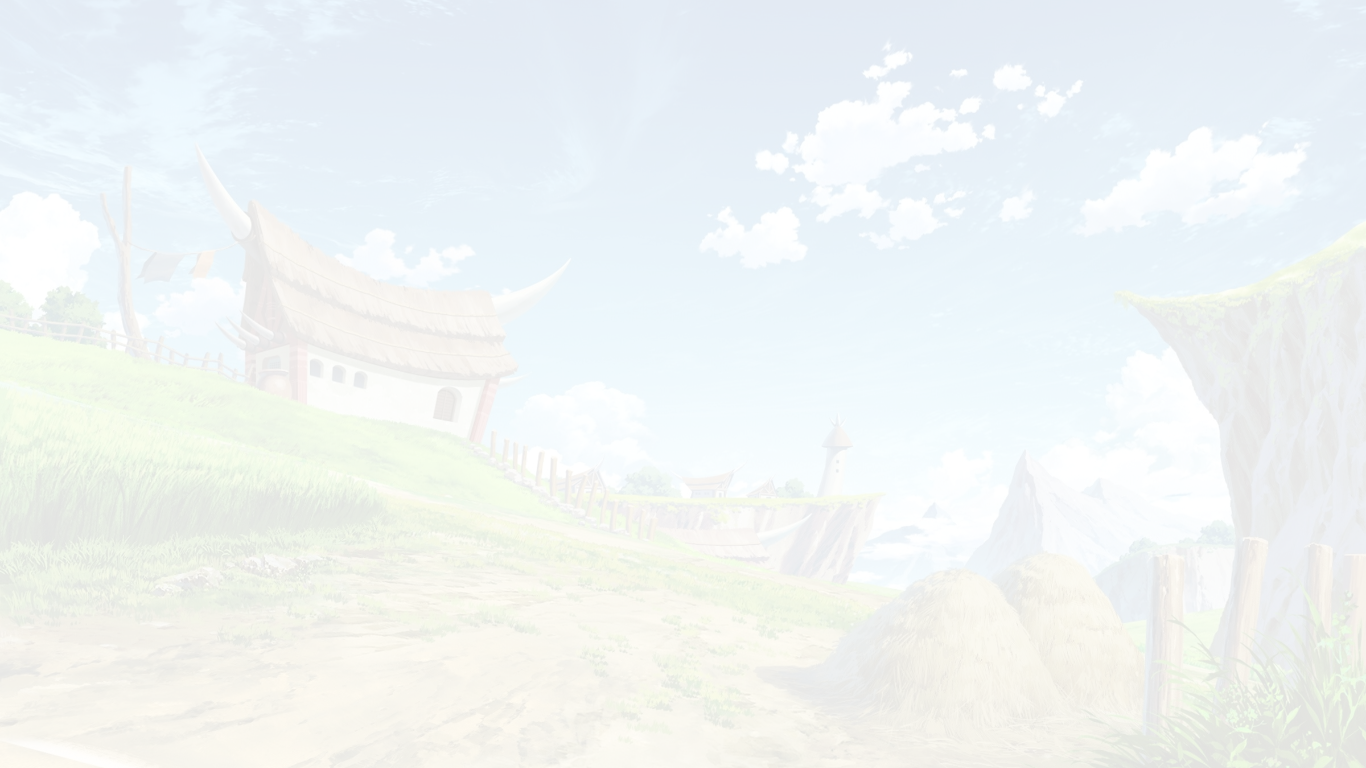
\includegraphics[width=\paperwidth]{4th-fleet.png}%
    }%
  }
}






\bigskip
\bigskip
\bigskip
\bigskip

\section{Mapping them against Knowledge, Skills and Behaviours}
\noindent This is a list of contents and mapped against the required knowledge, skills and behaviours I've been covering so far during the apprenticeship with ACL in Brentwood and on the workplace at Akhter Computers in Harlow Town:
%
%\begin{itemize}
%\item {Database development}
%\item {application life cycle}
%\item docker
%\item github 
%\item LateX
%\item PostgreSQL
%\item Linux
%\item {Mobile development}
%\end{itemize}
%

\medskip

\begin{tabular}{|c|c|}
    \hline
    \cellcolor{Azure2}\scalebox{1.5}{Database Development} & \cellcolor{Azure1}K1,K25 \\
    \hline
    \cellcolor{Azure3}\scalebox{1.5}{Android Development} & \cellcolor{Azure4}K24 \\
    \hline
    \cellcolor{Snow1}\scalebox{1.5}{Docker} & \cellcolor{Snow2}K5,K23 \\
    \hline
    \cellcolor{Snow3}\scalebox{1.5}{pgTAP} & \cellcolor{Snow4}K5 \\
    \hline
    \cellcolor{DarkSeaGreen1}\scalebox{1.5}{Github} & \cellcolor{DarkSeaGreen2}K15,K22 \\
    \hline
    \cellcolor{DarkSeaGreen3}\scalebox{1.5}{LateX} & \cellcolor{DarkSeaGreen4} \\
    \hline
    \cellcolor{Azure3}\scalebox{1.5}{Linux} & \cellcolor{Azure4}K14 \\
    \hline
\end{tabular}

\clearpage

\part{Mobile development}

In Figure \ref{fig:xamarin} we can see the stage I was on the 23rd March, with the mobile development. The progress of the whole thing is being quite slow since this is being literally self taught during my office hours

\begin{wrapfigure}[19]{r}{5cm}
\centering
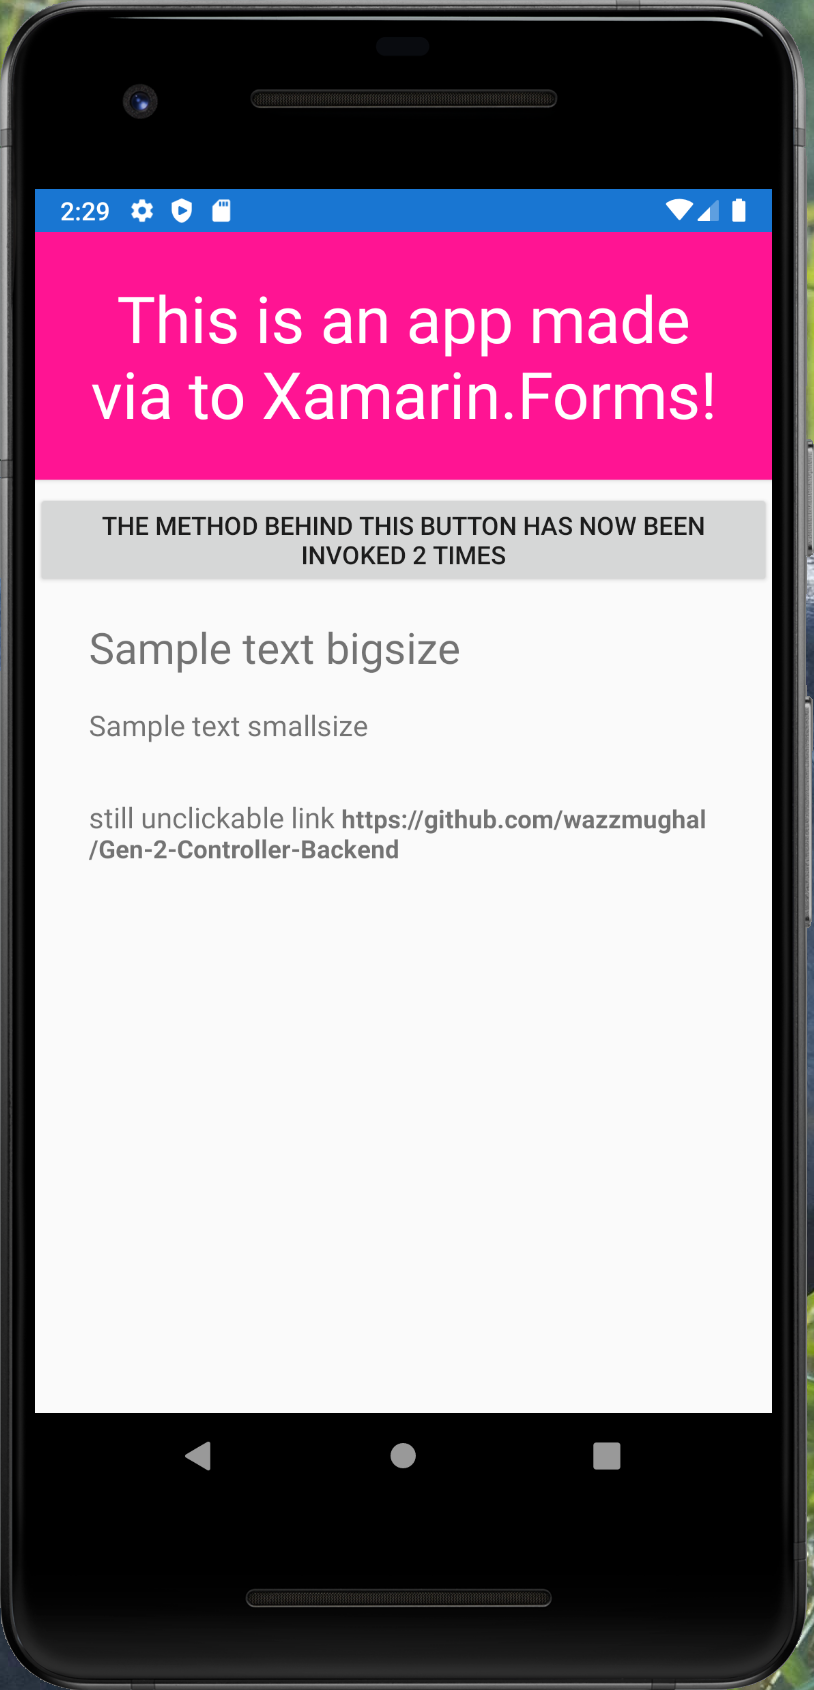
\includegraphics[width=4.8cm]{./capture-app.PNG}
%\hspace{-20pt}
\caption{Hello World in Xamarin with a button\footnotemark{}}\label{fig:xamarin}
\end{wrapfigure} 



We realized Xamarin brings in some difficulties even experts are struggling with. Since I'm on an apprenticeship we agreed to make it simple and use Android Studio to make an app for Android and later on use XCode for Apple. The problem with Apple is we'll need a real physical iPhone to test the app on.

After a little research I found out a tool called maptiler but it was going to be sunset soon so I've had to search more and I came up with \textbf{OSMDroid}

\bigskip
\bigskip

\scalebox{2}The next chapter shows how the app looks now on a Motorola g7(Figure \ref{fig:early}). Some functionalities have been added to test separately Client and Server functions. My app needs to interact with a C++ Server but because of the burden it takes to switch the real server on I've developed a quick server to have tests with and then once in a while see how it goes with the real server when it gets turned on.


\footnotetext{the button invokes an event saying how many times the user clicked it}

\chapter{Evidences from work}
%\AddToShipoutPictureBG*{
\includegraphics[width=\paperwidth,height=\paperheight]{wall.jpg}}

\AddToShipoutPictureBG*{%
  \AtPageUpperLeft{%
    \raisebox{-\height}{%
      
\includegraphics[width=\paperwidth]{wall.jpg}%
    }%
  }
}



\bigskip
\bigskip
\bigskip
\medskip
\medskip
\section{\scalebox{1.5}Milestone 05-May-2022}

\subsection{Targets}
%\bigskip
%\bigskip
%
\begin{itemize}
 \item{Login activity}
   \begin{description}
   \item[Messaging test]{Test how a hard coded GeoPosition can be sent through a socket from server to client}
   \item[Package visibility]{Make sure there is a way for the Login activity to pass informations to the MainActivity}
   \end{description}
 \item{nice user interface}
 \item{heavy testing against bugs}
 \item{calculation of middle position of all streetlight and having the map to start centered on that position}
 \item{iOS instance}
\end{itemize}

\clearpage

\subsection{Stage}

\begin{wrapfigure}[17]{r}{5cm}
%\centering
%\captionsetup{singlelinecheck=off, margin={6.67cm, 0cm}, justification=justified, format=hang}
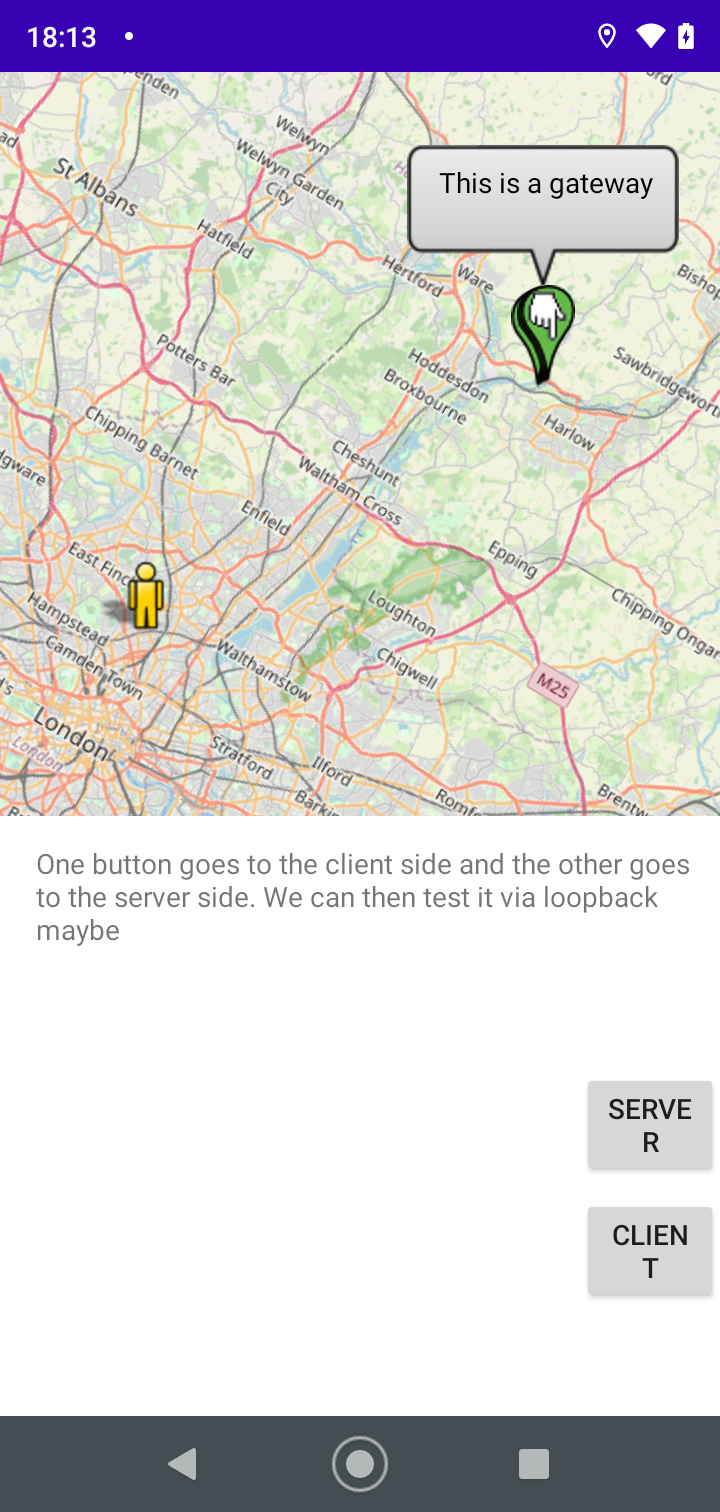
\includegraphics[width=4.4cm]{./current_status_g7.PNG}
%\vspace{-10pt}
\caption{User Interface on a Motorola g7}\label{fig:early}
\end{wrapfigure}

In Figure \ref{fig:early} you can find the stage I was at on the 5th of May where we're experimenting having the client and the server to talk to each other. The functionality it's still incapsulated in the client and needs to become part of the app rather than an external button. The Map at the beginning wasn't even rendering because proper permission needed to be handled in the Manifest.XML file. The the yellow man showing the actual position has been added using an Android built in function. The list of streetlights is still hardcoded and the first 3 are ItemizedOverlays whereas the last 3 are Markers.

Markers is the class we're inheriting from. The problem we have is to diplay on the map 3 different kinds of nodes:

\bigskip

\begin{itemize}
\item Streetlights
\item Gateway
\item {Gateways with Streetlight functionality}
\end{itemize}

\bigskip
for each one of these we want a different icon to be displayed. When using custom icons the problem we're still encountering is pinning. Custom icons don't get pinned as accurately as the default ones. We have switched to normal icons for the moment as the actual goal at the time of writing is to have an app that just works. Then we'll think to a nice user interface

\clearpage


\begin{wrapfigure}{L}{0.5\textwidth}
\centering
\includegraphics[width=4.5cm]{./server_g7.PNG}
%\vspace{-10pt}
\caption{server activity on a Motorola g7}\label{fig:connection-attempt}
\end{wrapfigure}
Figure \ref{fig:connection-attempt} shows how is the server activity doing on a Motorola while the client\footnotemark{} being run on a \textbf{Motorola g8 plus} attempts a connection to the server. As you can see, at the center of the app there is a TextView used as a temporary debug Console to debug the threads.

Debugging threads isn't always the easiest thing as you won't be following all of the in a single debug run so the decision has been taken to have them to print all the relevant information in a debugConsole. The problem is, when the debugConsole is full there's no way to read the past history.

To sort this out a scroll method has been added to the debugConsole

The little \textbf{CS} button on the top stands for Close Socket. It's a functionality is to close Socket where the messages are being sent.

\footnotetext{the client is being shown on Figure \ref{fig:connect-g8}}
%\arabic{WF@wrappedlines}
\wrapfill


\begin{wrapfigure}{R}{0.40\textwidth}
\centering\newcommand{\wrapfill}{\par\ifnum\value{WF@wrappedlines}>0
  \addtocounter{WF@wrappedlines}{-1}%
  \null\vspace{\arabic{WF@wrappedlines}\baselineskip}%
  \WFclear
\fi}
\includegraphics[width=4.5cm]{./client_g8.PNG}
%\vspace{-10pt}
\caption{client activity on a Motorola g8}\label{fig:connect-g8}
\end{wrapfigure}

The reason why I'm forcing the closure of the socket is to try figuring out how a nice communication can be realized between client and server and because at this stage is not possible to send more than one message I've introduced this functionality. The reason is because in the early stage no message was being sent at all and closing a socket solved the problem so I thought to do it again but this time it isn't of any help

Figure \ref{fig:connect-g8} shows how does it look the client activity on the Motorola g8 plus.Here we managed to connect to the server after the insertion of the Server IP address and port number. The problem is after sending one message the server receives it but no more messages are allowed

Because I was aware in advance of my ignorance and I had a so tarnished idea of how to realize all this I didn't embed the client-server communication in the app but kept it separate with buttons leading to other activities

These activities will be destroyed and I'll start new activities writing a simpler code that does just the bare minimum but guarantees the functionality
\wrapfill


\clearpage  

\begin{wrapfigure}[15]{R}{5cm}
\centering
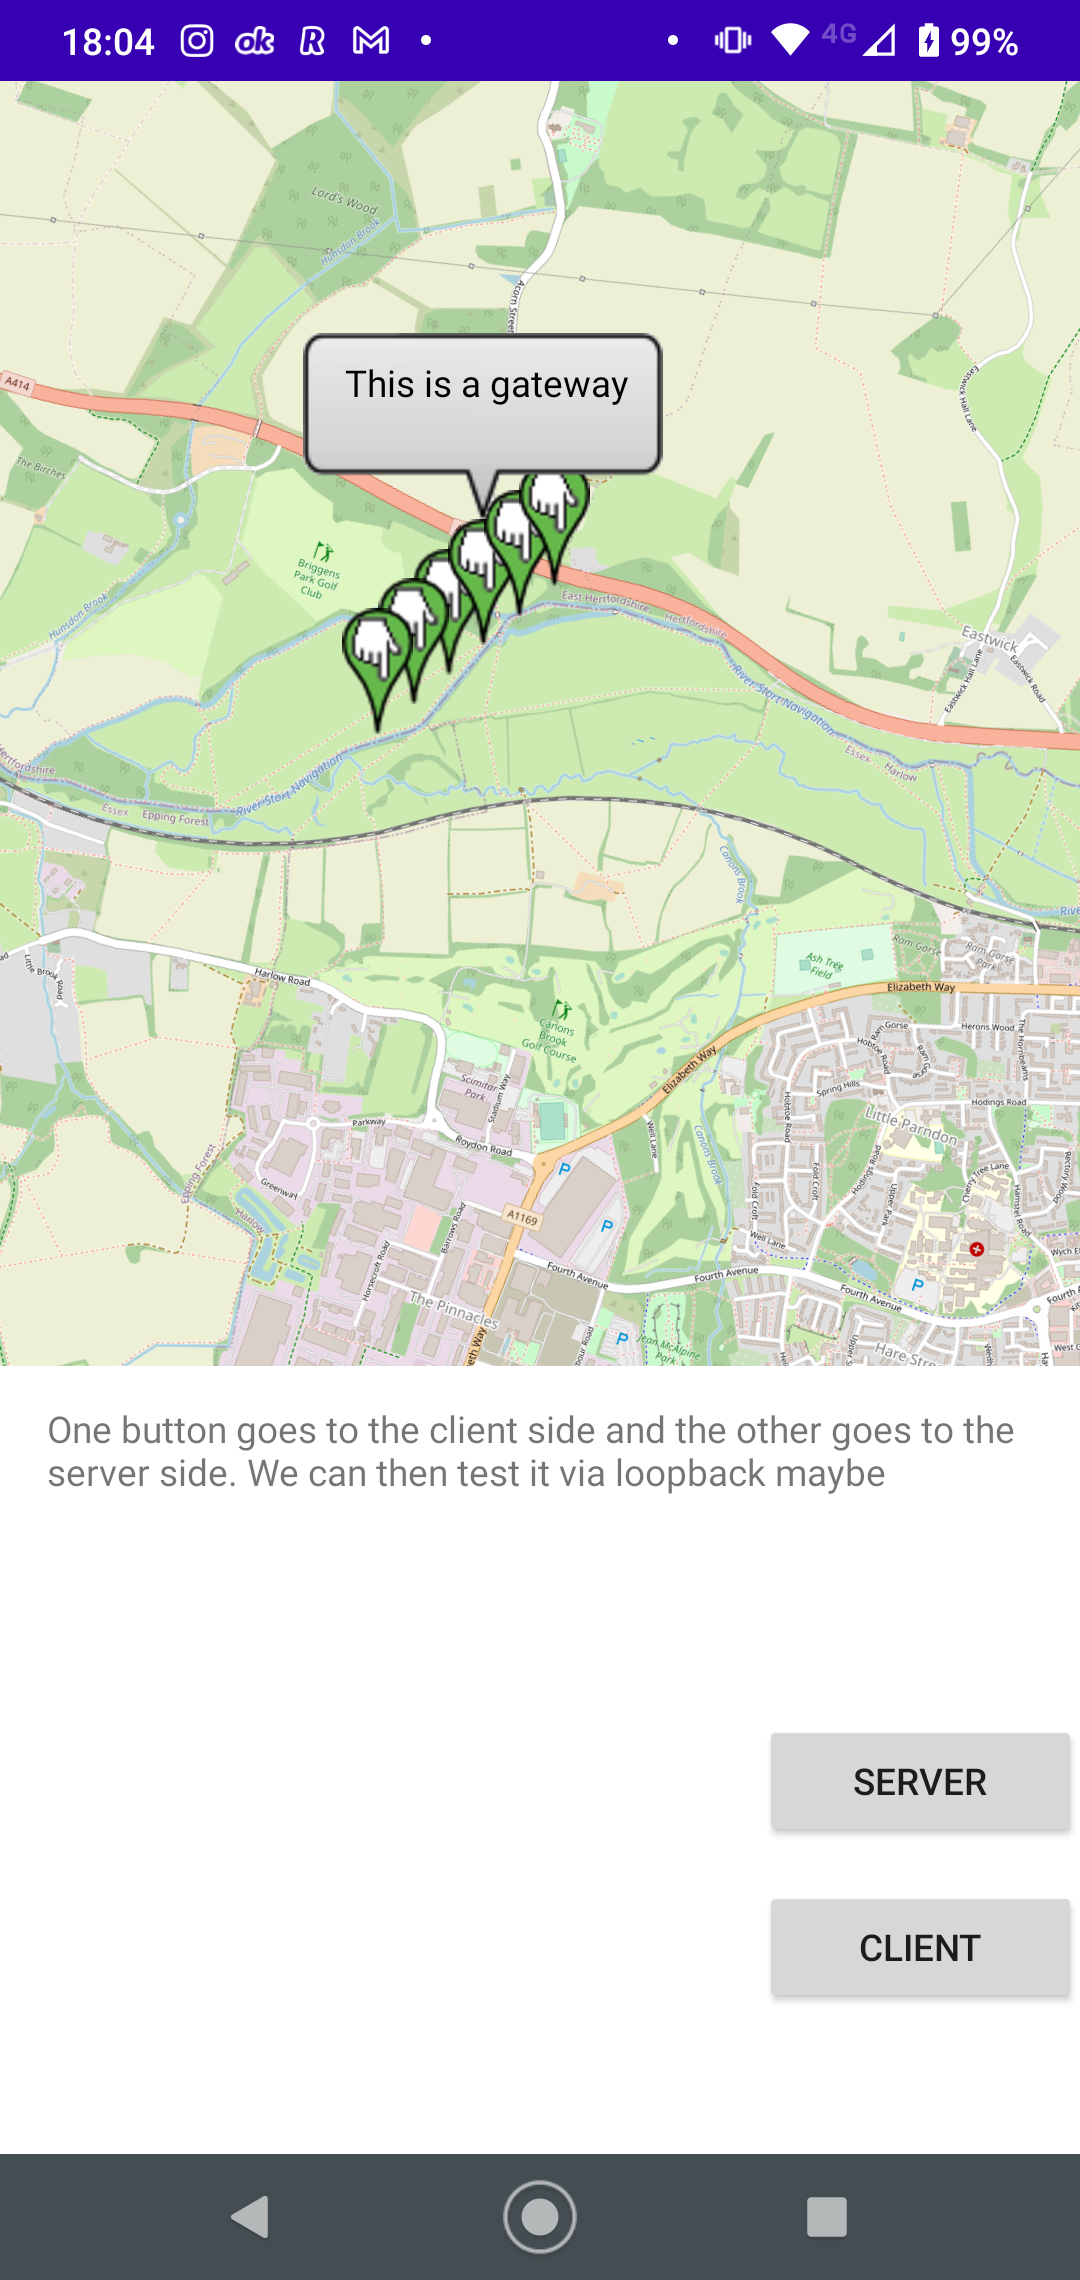
\includegraphics[width=4cm]{./current_status_g8.PNG}
%\vspace{-10pt}
\caption{User Interface on a Motorola g8}\label{fig:User-Interface-g8}
\end{wrapfigure}






And finally on Figure \ref{fig:User-Interface-g8} we can have a look at how the User Interface looks like on the Motorola g8. The phone model is wider than g7 so the text in the button is contained in one line only. This is due to how the Constraint View has been set. Is a minor problem and it will be sorted out in the future. But you definitely don't want to keep it like that after release.

Server button will be destroyed. The Server activity deleted. This is only to have something to test client's interactions with

Client activity will become the actual Login activity where the app picks

\clearpage
. 
\bigskip
\bigskip
\bigskip
\bigskip
\bigskip
\bigskip
\bigskip
\bigskip
\bigskip
\bigskip
\bigskip
\bigskip
\bigskip
\bigskip
\bigskip
\medskip
\medskip
\medskip
\section{\scalebox{1.5}Milestone 09-May-2022}

\AddToShipoutPictureBG*{%
  \AtPageUpperLeft{%
    \raisebox{-\height}{%
      
\includegraphics[width=\paperwidth]{wall.jpg}%
    }%
  }
}



\subsection{Targets}

\begin{itemize}
\item{Login activity}
   \begin{description}
   \item[\xout{Messaging test}]{\xout{Test how a hard coded GeoPosition can be sent through a socket from server to client}}
   \item[Package visibility]{Make sure there is a way for the Login activity to pass informations to the MainActivity}
   \end{description}
\item{nice user interface}
\item{heavy testing against bugs}
\item{calculation of middle position of all streetlight and having the map to start centered on that position}
\item{iOS instance}
\end{itemize}

\clearpage

\subsection{Stage}

\begin{wrapfigure}[19]{r}{4.81cm}
%\centering
%\captionsetup{singlelinecheck=off, margin={6.67cm, 0cm}, justification=justified, format=hang}
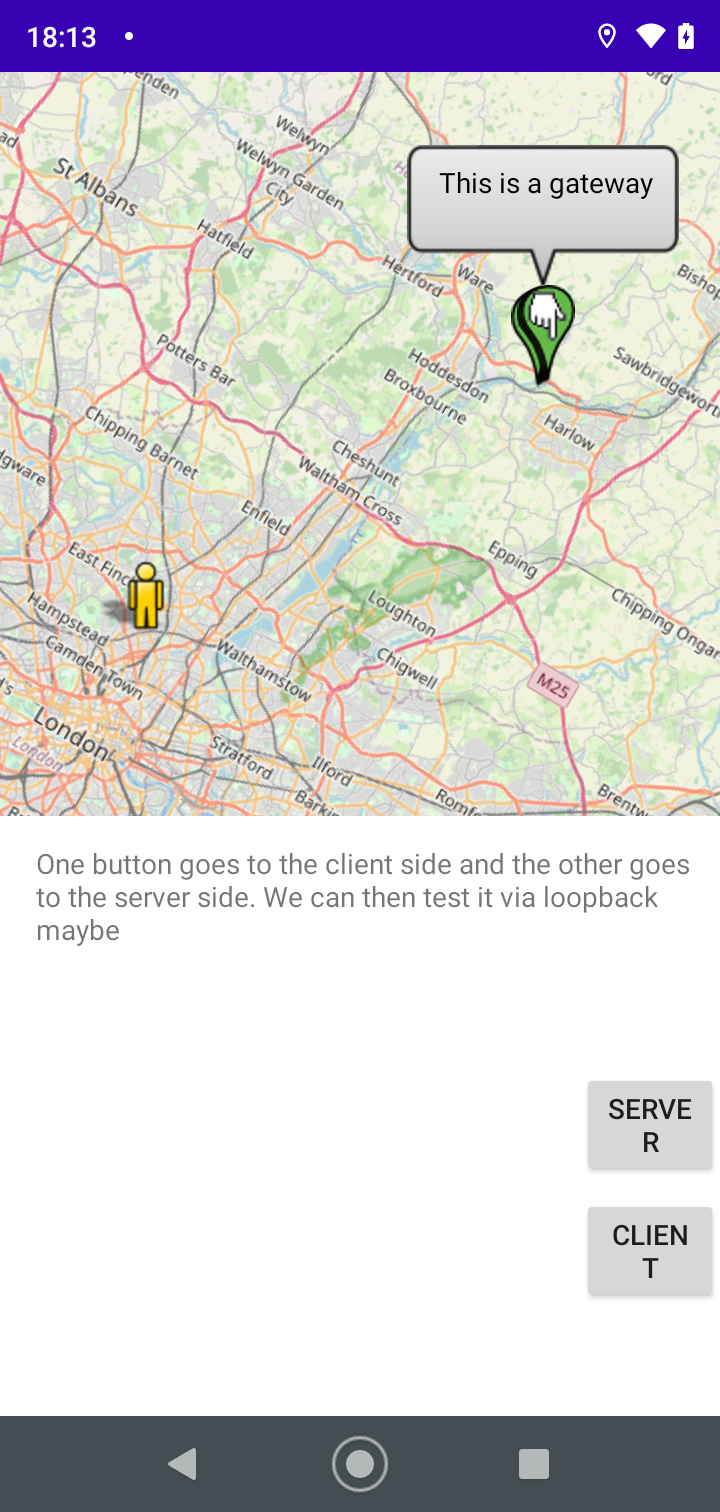
\includegraphics[width=4.4cm]{./current_status_g7.PNG}
%\vspace{-10pt}
\caption{User Interface on a Motorola g7}\label{fig:User-Interface-g7}
\end{wrapfigure}

In Figure \ref{fig:User-Interface-g7} you can find the stage I was at on the 9th of May where we were trying to have a hardcoded GeoPoint to travel through the socket and reach the client which will then pass it to the MainActivity and have it rendered on the map. This functionality it's still incapsulated in the client but will probably stay as it is and the buton will just be renamed to \textbf{Login}.

The problem is represented by chasing the information in the \emph{string} that comes out from the socket once the server has sent the information in it. Casting the String to a char[] array wouldn't work. Using the [] notation on a String doesn't work either to check all the element at once in a cycle. 


After spending the whole day asking my friends and doing research I found this code on the internet:

\begin{lstlisting}[language=java]
for(int i=0; i<s.length();i++)
{
  char c = s.charAt(i);
  System.out.println("char at "+i+"th index is: "+c);
}
\end{lstlisting}

but the code gives the error

\[ Could \ not \ resolve \ symbol: \ 's\ ' \]


\newline The reason of this is because I have used a name, which in this example is \emph{s}, that the compiler hasn't recognized.The compiler couldn't find the class.

So in other words this means that the Java compiler couldn't locate the symbol referenced in my Java code which in this case happens to be a variable named \emph{s}.

After a couple of phonecalls I got it solved by changing \emph{s} to \emph{line} bringing the code to become like so:

\begin{lstlisting}[language=java]
for(int i=0; i<line.length();i++)
{
  char c = line.charAt(i);
  System.out.println("char at "+i+"th index is: "+c);
}
\end{lstlisting}

\clearpage


\begin{wrapfigure}{L}{0.5\textwidth}
\centering
\includegraphics[width=4.5cm]{./9-May/server_g7.PNG}
%\vspace{-10pt}
\caption{server activity on a Motorola g7}\label{fig:server-activity-g7}
\end{wrapfigure}
Figure \ref{fig:server-activity-g7} shows how is the new server activity doing on a Motorola g7.

You can see it is listening on the port 8080. The IP here is not being shown as the WiFi Module just display what's in the Android Status so in order to know the device IP address I can just look there and reduce code usage which reduces crash chances. Not a lot of output is being displayed but we can safely assume it receives a connection and then closes the socket

The little \textbf{STOP} button on the top closes the Socket where the messages are being sent. Thus resulting in the client being unable to keep sending requests

The reason why that button is there is to simulate a server outage and see how the client behaves when the server is restarting.It's there to make the app robut against external failures by simply following the Boris Johnson\footnotemark{} approach against inflation living costs in 2022.

\footnotetext{making sure the system will work in the long run}
%\arabic{WF@wrappedlines}
\wrapfill


\begin{wrapfigure}{R}{0.40\textwidth}
\centering\newcommand{\wrapfill}{\par\ifnum\value{WF@wrappedlines}>0
  \addtocounter{WF@wrappedlines}{-1}%
  \null\vspace{\arabic{WF@wrappedlines}\baselineskip}%
  \WFclear
\fi}
\includegraphics[width=4.5cm]{./9-May/client_g8.PNG}
%\vspace{-10pt}
\caption{client activity on a Motorola g8}\label{fig:client-activity-g8}
\end{wrapfigure}

As you can see in Figure \ref{fig:client-activity-g8} the server is responding and the way to make it clear to the client as well is to send a 'SERVER RESPONDING' string through the socket. Then the client picks it up and drops it down on the debug Console.The DebugConsole as the name suggests is just there to really have an idea of what the threads are doing otherwise debugging them would be a real pain but in this way we can see on the screen just the messagges we feel relevant to the purpose.Then it Echoes a message 12345. This is because the client is sending 12345 to a C++ server as well which gets them in HEX format thus becoming 

\[ 3132333435aa \]

\noindent you can clearly see 1 becoming 31, 2 becoming 32 and so on. \textbf{aa} is probably the termination string or something but we know the C++ will always terminate its strings got via sockets with \textbf{aa}

\wrapfill

%\clearpage  

\noindent After that you can see the latitude and longitude being sent and received from the client which is what we wanted to obtain in the first place.One of the GOALS of the Target activity is thus accomplished.





\clearpage
. 
\bigskip
\bigskip
\bigskip
\bigskip
\bigskip
\bigskip
\bigskip
\bigskip
\bigskip
\bigskip
\bigskip
\bigskip
\bigskip
\bigskip
\bigskip
\medskip
\medskip
\medskip
\section{\scalebox{1.5}Crash on Login}

\AddToShipoutPictureBG*{%
  \AtPageUpperLeft{%
    \raisebox{-\height}{%
      
\includegraphics[width=\paperwidth]{wall.jpg}%
    }%
  }
}



\subsection{Targets}

\begin{itemize}
\item{Login activity}
   \begin{description}
   \item[\xout{Package visibility}]{\xout{Make sure there is a way for the Login activity to pass informations to the MainActivity}}
   \item[Crash on Login]{Understand what is causing the app to crash when the Login button is pressed}
   \end{description}
\item{nice user interface}
\item{heavy testing against bugs}
\item{calculation of middle position of all streetlight and having the map to start centered on that position}
\item{iOS instance}
\end{itemize}

\clearpage

\subsection{Stage}


We managed to understand how to pass data between activities in android and this is done by serializing data and literally adding it to the \textbf{Intent} but before I go on with the development of the app there's a problem I need to solve.

The app is crashing when the Login button is pressed. The crash is random and seems to be more frequent on devices with less RAM. Feels like a memory leak.

\subsection{Resolution}

To begin, the first I am doing is reducin the RAM available from 1.5Gb to 900Mb and as soon as I try to connect the client to the server I get another crash immediately. I have a look at the \href{https://github.com/danieledellacioppa/ACL-Assignments/blob/main/portfolio/verbose-logcat}{logcat} which on line 276 actually moans about something wasting RAM which could cause performance issue at startup

I had a look at this \href{https://github.com/danieledellacioppa/ACL-Assignments/blob/main/portfolio/2nd-verbose-logcat}{second logcat} generated as soon as I've got the same error again.
This logcat is really similar to the first one apart from a variable appearing as "?" on the first one and the last message it terminates with. This last message at line 400 in the second logcat is saying 

\[a \ resource \ failed \ to \ call \ close\]


After some research comes out this message was actually generated programmatically by this instruction: 

\begin{lstlisting}
System.logW("A resource failed to call "
        + (String) closerNameOrAllocationInfo + ". ");
\end{lstlisting}

The instruction just mentioned appears to be in this function named \textbf{warnIfOpen} :

\begin{lstlisting}
    public void warnIfOpen() {
        if (closerNameOrAllocationInfo != null) {
            if (closerNameOrAllocationInfo instanceof String) {
                System.logW("A resource failed to call "
                        + (String) closerNameOrAllocationInfo + ". ");
            } else {
                String message =
                        "A resource was acquired at attached stack trace but never released. ";
                message += "See java.io.Closeable for information on avoiding resource leaks.";
                Throwable stack = (Throwable) closerNameOrAllocationInfo;
                reporter.report(message, stack);
            }
        }
    }
\end{lstlisting}

After running the app on the mobile with 1 Gb RAM \footnote{\label{mobile-crash} this test is being run against the android server instead of the C++ one so the result might be different. The reason is because the Android Server is the only thing I can have on the same wifi at the moment. I don't have my laptop at the moment otherwise I'd have installed the C++ server on the laptop and logged on the same wifi} the logcat shows:

\begin{lstlisting}
2022-07-05 11:36:45.183 4217-4217/? I/mdroid_app_jav: Late-enabling -Xcheck:jni
2022-07-05 11:36:45.213 4217-4217/? E/mdroid_app_jav: Unknown bits set in runtime_flags: 0x8000
2022-07-05 11:36:45.632 4217-4217/com.example.osmdroid_app_java I/StorageUtils: /data/user/0/com.example.osmdroid_app_java/files is writable
2022-07-05 11:36:45.638 4217-4217/com.example.osmdroid_app_java I/StorageUtils: /storage/emulated/0/Android/data/com.example.osmdroid_app_java/files is writable
2022-07-05 11:36:45.639 4217-4217/com.example.osmdroid_app_java I/StorageUtils: /data/user/0/com.example.osmdroid_app_java/files is writable
2022-07-05 11:36:45.640 4217-4217/com.example.osmdroid_app_java I/StorageUtils: /storage/emulated/0/Android/data/com.example.osmdroid_app_java/files is writable
2022-07-05 11:36:45.670 4217-4217/com.example.osmdroid_app_java I/OsmDroid: Using tile source specified in layout attributes: Mapnik
2022-07-05 11:36:45.670 4217-4217/com.example.osmdroid_app_java I/OsmDroid: Using tile source: Mapnik
2022-07-05 11:36:45.675 4217-4217/com.example.osmdroid_app_java I/OsmDroid: Tile cache increased from 0 to 9
2022-07-05 11:36:45.855 4217-4251/com.example.osmdroid_app_java I/AdrenoGLES: QUALCOMM build                   : 961b24f, Ib57168459a
    Build Date                       : 02/24/20
    OpenGL ES Shader Compiler Version: EV031.27.05.06
    Local Branch                     : 
    Remote Branch                    : 
    Remote Branch                    : 
    Reconstruct Branch               : 
2022-07-05 11:36:45.855 4217-4251/com.example.osmdroid_app_java I/AdrenoGLES: Build Config                     : S L 8.0.12 AArch32
2022-07-05 11:36:45.859 4217-4251/com.example.osmdroid_app_java I/AdrenoGLES: PFP: 0x005ff113, ME: 0x005ff066
2022-07-05 11:36:45.879 4217-4217/com.example.osmdroid_app_java I/OsmDroid: Tile cache increased from 9 to 12
2022-07-05 11:36:45.900 4217-4251/com.example.osmdroid_app_java W/Gralloc3: mapper 3.x is not supported
\end{lstlisting}

\[mapper \ 3.x \ is \ not \ supported\]

On \href{https://github.com/flutter/flutter/issues/50405}{this forum} they're talking about it and they're talking about a crash which is encouraging.But running the test again now this bit gets my attention:

\[Unknown \ bits \ set \ in \ runtime\_flags: \ 0x8000\]

This is literally the second line of the logcat and has \textbf{E/mdroid\_app\_jav} meaning it is indeed an error \footnote{\label{error} Because it starts with E}.

On \href{https://stackoverflow.com/questions/56916587/unknown-bits-set-in-runtime-flags-0x8000-warning-in-logcat-on-android-q-emula}{this forum} someone suggested to use this:

\begin{lstlisting}

@Override
public void onStop() {
    super.onStop();
    getActivity().finish();
}

\end{lstlisting}

But getActivity() is not found.After some research I've found out an Activity has no getActivity() method.Fragments have. Because getActivity() says: "return the Activity which contains me".And while Framents are contained in Activities, Activities themselves aren't. I guess I'll just use this.finish() instead. Should be fine. Meaning my code will be:

\begin{lstlisting}

@Override
public void onStop() {
    super.onStop();
    this.finish();
}

\end{lstlisting}

After managing the java.net.NoRouteToHostException works fine fore a while but then pressing the \textsc{connect to server} button a few times in a row still gives me the same crash with the same log:

\begin{lstlisting}
2022-07-05 14:36:36.462 9236-9236/? I/mdroid_app_jav: Late-enabling -Xcheck:jni
2022-07-05 14:36:36.492 9236-9236/? E/mdroid_app_jav: Unknown bits set in runtime_flags: 0x8000
2022-07-05 14:36:36.931 9236-9236/com.example.osmdroid_app_java I/StorageUtils: /data/user/0/com.example.osmdroid_app_java/files is writable
2022-07-05 14:36:36.936 9236-9236/com.example.osmdroid_app_java I/StorageUtils: /storage/emulated/0/Android/data/com.example.osmdroid_app_java/files is writable
2022-07-05 14:36:36.937 9236-9236/com.example.osmdroid_app_java I/StorageUtils: /data/user/0/com.example.osmdroid_app_java/files is writable
2022-07-05 14:36:36.938 9236-9236/com.example.osmdroid_app_java I/StorageUtils: /storage/emulated/0/Android/data/com.example.osmdroid_app_java/files is writable
2022-07-05 14:36:36.974 9236-9236/com.example.osmdroid_app_java I/OsmDroid: Using tile source specified in layout attributes: Mapnik
2022-07-05 14:36:36.974 9236-9236/com.example.osmdroid_app_java I/OsmDroid: Using tile source: Mapnik
2022-07-05 14:36:36.980 9236-9236/com.example.osmdroid_app_java I/OsmDroid: Tile cache increased from 0 to 9
2022-07-05 14:36:37.168 9236-9275/com.example.osmdroid_app_java I/AdrenoGLES: QUALCOMM build                   : 961b24f, Ib57168459a
    Build Date                       : 02/24/20
    OpenGL ES Shader Compiler Version: EV031.27.05.06
    Local Branch                     : 
    Remote Branch                    : 
    Remote Branch                    : 
    Reconstruct Branch               : 
2022-07-05 14:36:37.168 9236-9275/com.example.osmdroid_app_java I/AdrenoGLES: Build Config                     : S L 8.0.12 AArch32
2022-07-05 14:36:37.175 9236-9275/com.example.osmdroid_app_java I/AdrenoGLES: PFP: 0x005ff113, ME: 0x005ff066
2022-07-05 14:36:37.190 9236-9236/com.example.osmdroid_app_java I/OsmDroid: Tile cache increased from 9 to 12
2022-07-05 14:36:37.207 9236-9275/com.example.osmdroid_app_java W/Gralloc3: mapper 3.x is not supported
\end{lstlisting}

\part{Database development}

The followings are the tasks I'm responsible with databases. You can label it the way you want but it's pretty much the whole lifecycle management except \emph{talking to the client}, make sure we both agree on \emph{what they want}, \emph{writing the specs} of the solution that needs to be \emph{designed}.

Hence my list of responsibilites with the database covers:

\begin{itemize}
\item {reading the specs}
\item design
\item implementation
\item testing 
\item documenting
\end{itemize}

\clearpage

\chapter{Database design}
This is a first idea of the database I came up with

\noindent\includegraphics[width=14cm]{./ERSchemaGen2.jpg}

We agreed it was holding probably more information than what we need to display in the app so I came up later on with a smaller design which really has just the right amount of things we need to make sure we can run enough tests and see how the App, the Server and the Database interact between each other
\clearpage

This is the smaller database designed again from scratch. We need to add geolocation to nodes but for the time being it will be hard coded in the server and we'll try to see if we can display a hardcoded geolocation hold by the server to be caught by the client and displayed properly on the app

\noindent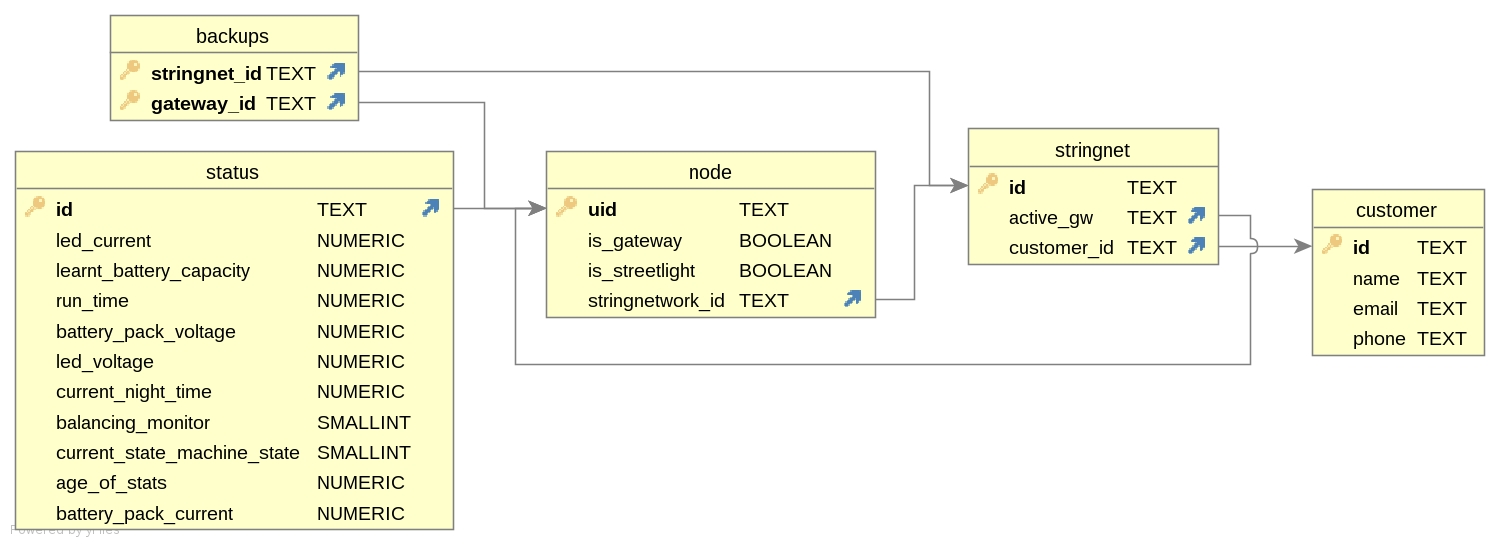
\includegraphics[width=14cm]{./SecondERSchemaGen2.jpg}

\printindex

\end{document}
